\documentclass[10pt]{article}
\usepackage[top=0.45in,bottom=0.42in,left=0.65in,right=0.65in]{geometry}
\usepackage{amsmath,amssymb}
\usepackage{graphicx}
\usepackage{caption}
\usepackage{xcolor}
\usepackage{microtype}
\usepackage{booktabs}
\definecolor{navy}{HTML}{1F3A5F}
\newcommand{\bg}{\kern0.05em\textcolor{white}{.}\kern0.05em\allowbreak}
\newcommand{\sect}[1]{\vspace{0pt}\noindent{\bfseries\color{navy}#1}\par\nobreak\vspace{-1pt}}
\captionsetup{font=footnotesize,labelfont={bf,color=navy},skip=4pt,
              justification=raggedright,singlelinecheck=false}
\setlength{\parskip}{1pt}
\setlength{\parindent}{0pt}
\setlength{\abovedisplayskip}{1pt}\setlength{\belowdisplayskip}{1pt}
\setlength{\abovedisplayshortskip}{0pt}\setlength{\belowdisplayshortskip}{0pt}
\pagestyle{empty}
\renewcommand{\topfraction}{.97}\renewcommand{\bottomfraction}{.97}
\renewcommand{\textfraction}{.03}\renewcommand{\floatpagefraction}{.92}

\newcommand{\Pts}{\mathrm{Pts}}
\newcommand{\FGpct}{\mathrm{FG\%}}
\newcommand{\FTpct}{\mathrm{FT\%}}
\newcommand{\FTrate}{\mathrm{FT\,rate}}
\newcommand{\prop}{\mathrm{prop}}
\newcommand{\PPG}{\mathrm{PPG}}
\newcommand{\PtsFGA}{\mathrm{Pts/FGA}}
\begin{document}
\begin{center}
{\Large\bfseries\color{navy} Jimmies and Joes or X's and O's?\\[1pt]
More Risk for Less Return in Modern NBA Shot-Selection}\\[3pt]
{\large\bfseries An ML and Markowitz Portfolio Analysis of $2^{nd}$-Order Shot\\[1pt]
Statistics in a $1^{st}$-Order Analytic League}\\[4pt]
{\small Word Count: 496; Track: Basketball; Github: github.com/sdsander-syr/MIT-SSAC-NBA-Risk-Return-Shot-Portfolio/upload/main }
\end{center}
\vspace{1pt}

\sect{1. Introduction}
\noindent
The first-wave of basketball analytics has focused almost exclusively on
first-order statistics. But first-order results are often \emph{average}, obscuring deviance.
We should \emph{expect} more. By first-order logic, the \emph{St. Petersburg Paradox} presents unboundedly-high ROI for any finite entry-fee (Bernoulli, 1738). A first-order maximizer accepts the bet at any earthly entry-fee. Yet, most won't commit their lunch money for entry (Hayden and Platt, 2009). Risk also matters in NBA basketball despite the League's bounded-ROI. Game-level scoring-risk is substantial, and should be second-order only statistically. NBA teams compete for game-wins, not season-table-wins, given a statistically-moderate number of game-possessions; scoring-variance is substantial and directly-linked to shooting-ability and shot-selection, the latter a short-run choice-variable.

\sect{2. Methods}
\noindent
\textbf{Shot-portfolio variance} is a point-value-weighted sum of binomial-variances for each FGA and FGA-pursuant FTA, both linked to the original FGA-type/zone-location, and \textbf{shot-portfolio return} follows from the same inputs:
\begin{align}
\sigma^{2}\;&=\;n\sum_{z=1}^{Z}\prop_{z}\cdot\Bigl[\,\Pts_{z}^{2}\cdot\FGpct_{z}\cdot\bigl(1-\FGpct_{z}\bigr)\;+\;\FTrate_{z}\cdot\FTpct\cdot\bigl(1-\FTpct\bigr)\Bigr],\\[1pt]
\PtsFGA_{z}\;&=\;\Pts_{z}\cdot\FGpct_{z}+\FTrate_{z}\cdot\FTpct,\qquad
\PPG\;=\;n\sum_{z=1}^{Z}\prop_{z}\cdot\PtsFGA_{z}.
\end{align}
where $z$ is shot-type/zone-location, $n$ is FGAs per team-game, $\prop_{z}$ the type-conditional shot-frequency, $\Pts_{z}\in\{2,3\}$ is attempt point-value, $\FGpct_{z}$ the zone-conditional conversion-rate, $\FTrate_{z}$ the zone-conditional shot-pursuant FT-rate, and $\FTpct$ FT-accuracy, so that $(\FTrate_{z}\cdot\FTpct)$ is zone-conditional made FT-rate.
We treat NBA team-game shot-selection as a portfolio of heterogeneous Bernoulli-trials differing in zone-distribution and thus in points-expectation, scoring-risk/variance, and shot-pursuant FT-rate, where unfouled 3PA (2PA) variance scales by 9 (4). Using modern, \textbf{Markowitz portfolio-theory} from finance, \textbf{step-linear programming}, and \textbf{GAM-ML modeling}, we model first- \emph{and} second-order shot-selection statistics to determine how \emph{expected} are game-level expectations. \textbf{Each shot-portfolio} has a \textbf{quantifiable risk-return signature}. The risk-return efficient shot-selection frontier solves a step-linear program. Risk is the ``bad'' input and scoring the ``good'' output. Both moments depend on the cross-zone attempt-share vector, $\prop=(\prop_{1},\dots,\prop_{Z})$. A portfolio's quality is the ordered-pair $RiskReturn(\prop)=\bigl(\sigma(\prop),\bar{PPG}(\prop)\bigr)\in\mathbb{R}_{+}^{2}$ in the risk-return Cartesian-plane, and season-$t$ league-frontier is the attainable set's upper-envelope for a league-representative team,
\begin{equation}
F_{t}(s)\;=\;\max_{\prop\,\in\,\Delta^{Z-1}}\bigl\{\,\PPG_{t}(\prop)\ :\ \sigma_{t}(\prop)\le s\,\bigr\},
\qquad
\Delta^{Z-1}=\Bigl\{\prop\in\mathbb{R}_{+}^{Z}:\ \sum\nolimits_{z=1}^{Z}\prop_{z}=1\Bigr\}.
\end{equation}
The \textbf{Markowitz-frontier} allows for no attainable pair to its northwest. Partitioning the offensive-floor into six zones over 390 team-seasons from 2013-14---2025-26, the 30-stadium tracking-era, a GAM-ML model learns the efficiency-frontier for each season by inputting 2{,}340 zone/team/season trios, fitting \textbf{attempt-weighted, ridge-penalized cubic-splines smoothed} in season, team FT-accuracy (exogenous shooting-skill), and pace. A box-score identity yields each shot-type's shot-pursuant FT-scoring value. Accordingly, \textbf{Fig.1} visualizes the \textbf{$\sim$2.77-million FGAs} from 2013-26. 

\noindent\begin{minipage}{\textwidth}\centering
\begin{minipage}[c]{0.470\textwidth}\centering
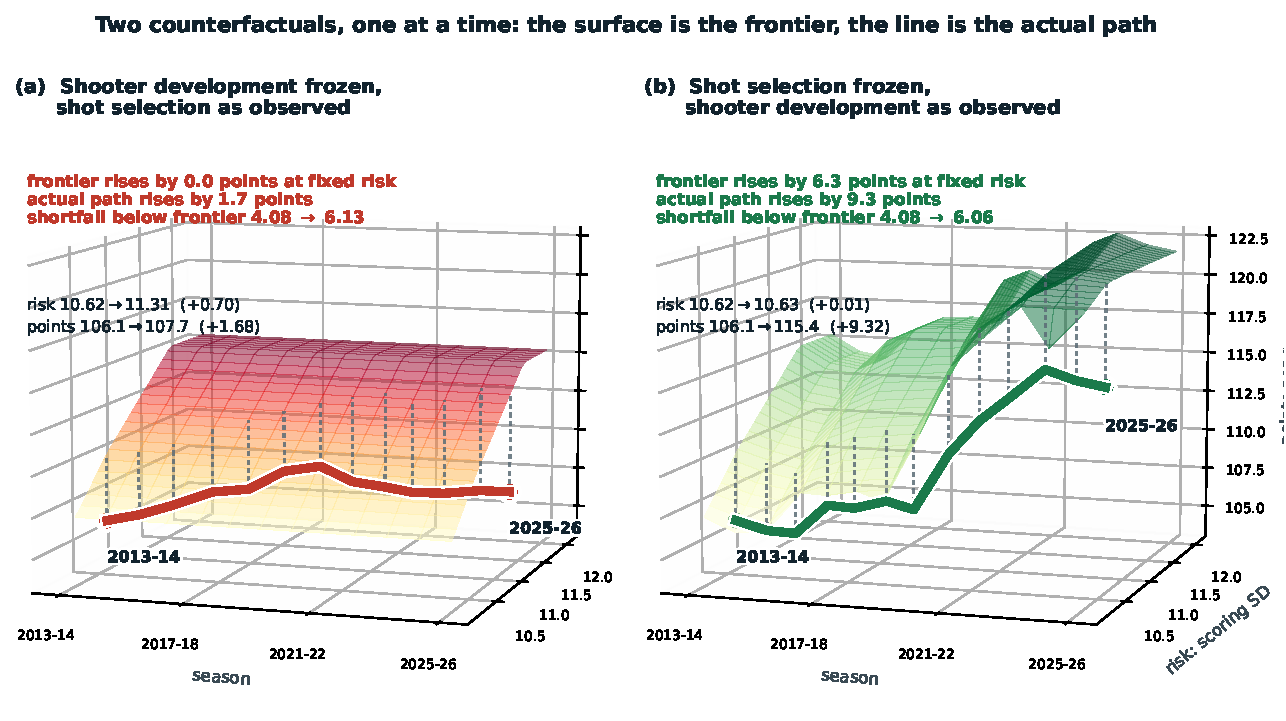
\includegraphics[width=\linewidth]{cf3d (1).pdf}
\end{minipage}\hfill
\begin{minipage}[c]{0.515\textwidth}\centering
{\fontsize{5.8}{6.7}\selectfont\setlength{\tabcolsep}{2.5pt}\renewcommand{\arraystretch}{0.82}
\begin{tabular}{@{}lrrr@{}}
\toprule
 & $\Delta$\bg Shooter & $\Delta$\bg SD\bg of & Vertical \\
 & Develop- & Team-Game & Expected\bg Pts. \\
 & ment\bg Gain & Pts. & Lost,\bg Shot-Sel. \\
Season & & & Inefficiency \\
\midrule
2013\bg--14 & +0.00 & +0.00 & 4.08 \\
2014\bg--15 & -0.56 & +0.04 & 4.03 \\
2015\bg--16 & -0.58 & +0.11 & 3.41 \\
2016\bg--17 & +1.21 & +0.26 & 3.78 \\
2017\bg--18 & +1.25 & +0.35 & 4.69 \\
2018\bg--19 & +1.75 & +0.44 & 4.03 \\
2019\bg--20 & +1.45 & +0.55 & 4.61 \\
2020\bg--21 & +4.80 & +0.59 & 5.71 \\
2021\bg--22 & +6.92 & +0.64 & 6.53 \\
2022\bg--23 & +8.42 & +0.58 & 6.08 \\
2023\bg--24 & +10.10 & +0.61 & 6.35 \\
2024\bg--25 & +9.54 & +0.72 & 6.83 \\
2025\bg--26 & +9.32 & +0.70 & 6.68 \\
\bottomrule
\end{tabular}}
\end{minipage}
\captionof{figure}{For \bg each \bg plot of Fig.1, the\bg surface\bg is\bg the\bg frontier,\bg and\bg the\bg line\bg is\bg the\bg actual\bg path.\bg Left\bg panel:\bg Shooter\bg development\bg frozen\bg at\bg 2013-14\bg with\bg shot\bg selection\bg as\bg observed over time.\bg Right\bg panel:\bg Shot\bg selection\bg frozen\bg with\bg shooter\bg development\bg as\bg observed over time. The frontiers show that offensive shooting efficiency gains were driven by shooter-development, which rose dramatically. Shot-selection became more inefficient (further inside of an improving shot-development frontier) over time. Shooter-development is the general ability of players to shoot from randomly-selected locations, and shot-selection is the ability of players to select hot-spot locations.}
\end{minipage}
\vspace{3pt}

\noindent\begin{minipage}{\textwidth}\centering
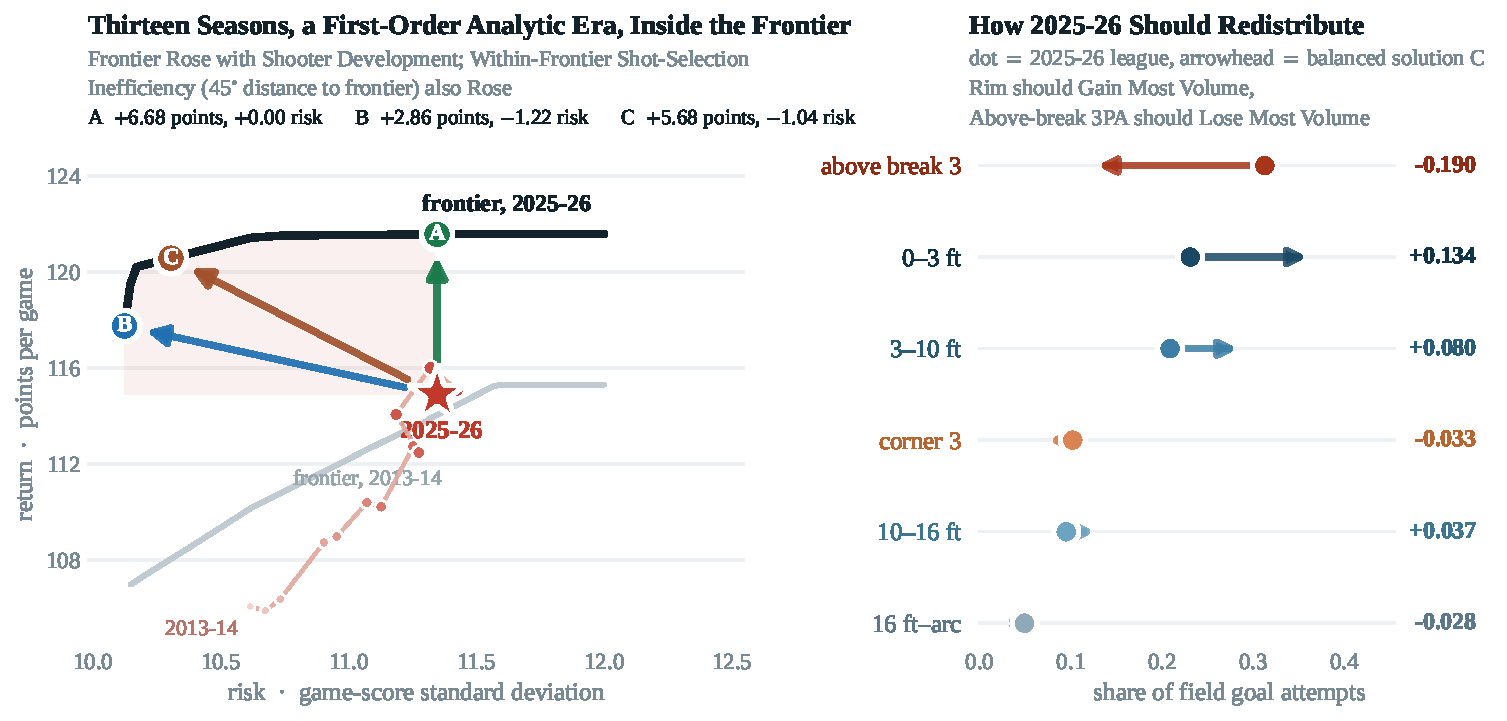
\includegraphics[width=0.60\textwidth]{arbitrage (5).pdf}\\[4pt]
\begin{minipage}[t]{0.495\textwidth}\centering
{\scriptsize\textbf{2013-14\bg through\bg 2025-26\bg Shot\bg Selection\bg Data\bg Summary}}\\[2pt]
{\fontsize{5.2}{6.0}\selectfont\setlength{\tabcolsep}{1.8pt}\renewcommand{\arraystretch}{0.90}
\begin{tabular}{@{}lrrrrr@{}}
\toprule
Zone & Attempts & Share & $\theta$ & Exp.\bg Pts. & SD \\
\midrule
above\bg break\bg 3 & 755{,}379 & 27.2\% & 0.171 & 1.220 & 1.444 \\
0\bg--3\bg ft & 736{,}316 & 26.5\% & 0.219 & 1.549 & 0.970 \\
3\bg--10\bg ft & 501{,}631 & 18.1\% & 0.223 & 1.070 & 1.014 \\
16\bg ft\bg--arc & 280{,}111 & 10.1\% & 0.214 & 1.010 & 1.004 \\
10\bg--16\bg ft & 271{,}812 & 9.8\% & 0.220 & 1.062 & 1.013 \\
corner\bg 3 & 230{,}492 & 8.3\% & 0.169 & 1.331 & 1.474 \\
\midrule
\textbf{Total\bg FGA} & \textbf{2{,}775{,}740} & \textbf{100.0\%} & \textbf{0.202} & \textbf{1.253} & \textbf{1.177} \\
\multicolumn{6}{@{}l@{}}{\fontsize{5.2}{6.0}\selectfont zone-share\bg $=-0.071+0.223\,$Exp.Pts.$\,-0.028\,$SD,\bg\bg $R^{2}=0.273$} \\
\multicolumn{6}{@{}l@{}}{\fontsize{5.2}{6.0}\selectfont zone-share\bg $=-0.095+0.217\,$Exp.Pts.,\bg\bg $R^{2}=0.267$} \\
\multicolumn{6}{@{}l@{}}{\fontsize{5.2}{6.0}\selectfont zone-share\bg $=+0.153+0.012\,$SD,\bg\bg $R^{2}=0.001$} \\
\bottomrule
\end{tabular}}
\end{minipage}\hfill
\begin{minipage}[t]{0.465\textwidth}\centering
{\scriptsize\textbf{2025-26\bg Shot\bg Selection\bg Data\bg Summary}}\\[2pt]
{\fontsize{5.2}{6.0}\selectfont\setlength{\tabcolsep}{1.8pt}\renewcommand{\arraystretch}{0.90}
\begin{tabular}{@{}lrrrrr@{}}
\toprule
Zone & Attempts & Share & $\theta$ & Exp.\bg Pts. & SD \\
\midrule
above\bg break\bg 3 & 68{,}675 & 31.3\% & 0.124 & 1.175 & 1.441 \\
0\bg--3\bg ft & 50{,}758 & 23.1\% & 0.250 & 1.662 & 0.941 \\
3\bg--10\bg ft & 45{,}887 & 20.9\% & 0.250 & 1.171 & 1.024 \\
corner\bg 3 & 22{,}439 & 10.2\% & 0.124 & 1.284 & 1.470 \\
10\bg--16\bg ft & 20{,}887 & 9.5\% & 0.250 & 1.137 & 1.021 \\
16\bg ft\bg--arc & 10{,}835 & 4.9\% & 0.250 & 1.045 & 1.006 \\
\midrule
\textbf{Total\bg FGA} & \textbf{219{,}481} & \textbf{100.0\%} & \textbf{0.198} & \textbf{1.288} & \textbf{1.201} \\
\multicolumn{6}{@{}l@{}}{\fontsize{5.2}{6.0}\selectfont zone-share\bg $=-0.238+0.202\,$Exp.Pts.$\,+0.133\,$SD,\bg\bg $R^{2}=0.245$} \\
\multicolumn{6}{@{}l@{}}{\fontsize{5.2}{6.0}\selectfont zone-share\bg $=-0.055+0.178\,$Exp.Pts.,\bg\bg $R^{2}=0.148$} \\
\multicolumn{6}{@{}l@{}}{\fontsize{5.2}{6.0}\selectfont zone-share\bg $=+0.049+0.102\,$SD,\bg\bg $R^{2}=0.059$} \\
\bottomrule
\end{tabular}}
\end{minipage}
\captionof{figure}{Left:\bg the\bg league's\bg thirteen-season\bg path,\bg pale\bg to\bg red,\bg against\bg the\bg 2013-14\bg and\bg 2025-26\bg frontiers,\bg with\bg the\bg 2025-26\bg portfolio\bg starred\bg and\bg improvement\bg directions\bg A,\bg B,\bg C;\bg the\bg shaded\bg region\bg holds\bg every\bg allocation\bg beating\bg it\bg on\bg both\bg axes.\bg Right:\bg share\bg of\bg attempts\bg by\bg zone,\bg from\bg the\bg 2025-26\bg league\bg (dot)\bg to\bg balanced\bg solution\bg C\bg (arrowhead).\bg Below,\bg attempt-weighted:\bg theta\bg is\bg shot-pursuant\bg free-throw\bg value\bg per\bg attempt,\bg expected\bg points\bg adds\bg it\bg to\bg field-goal\bg value,\bg SD\bg is\bg scoring\bg standard\bg deviation\bg per\bg attempt.}
\end{minipage}
\vspace{3pt}


\enlargethispage{7\baselineskip}%
\sect{3. Results}
\noindent
\textbf{Shooter-development}, estimated by League conversion-rate across floor-zones without weighting for location-conditional volume, \textbf{rose by 9.32 ppg from 2013-26}. This pushed the efficiency frontier out accordingly. The League moved up and to the right (from dot-to-star in left panel of Fig.2), accepting more risk for additional points. However, shot-selection inefficiency, vertical-distance within season-level frontier, \textbf{rose from 4.08 points to 6.68 points} (Fig.1), 2.6-ppg more inefficient. Moreover, team-game shot-portfolios gained 0.70 additional points of standard-deviation (scoring-risk). \textbf{Shooting became better, but only because of development and in spite of growing shot-selection inefficiency.} At-the-rim returns $1.662$ points per attempt at $0.941$ standard deviation, the highest-return and lowest risk zone; Above-the-break 3PAs return $1.175$ at $1.441$ on $31.3$-percent of FGAs against $23.1$-percent at-the-rim. The latter zone-share has fallen over the sample despite risk-return dominance. and the former has risen. Fig.2 shows that, from 2013-26 overall, NBA teams increased shot-volume with greater zone-return but shot-volume didn't respond to zone-risk. By 2025-26, zone-volume increased less strongly in zone-return than previously, and NBA players were \textbf{more likely to seek high-risk over low-risk zones for the same return}! This is what came of a data revolution. Teams became worse at finding hot-return zones, and more actively sought hot-risk zones. Consequently, risk and return now explain less of the variation in zone-level shot-volume than in 2013. These regressions demonstrate substantial shot-selection efficiency \emph{regression}! 

\sect{4. Conclusion}
\noindent
The modern NBA is thus nowhere near its shot-selection frontier. Analytics staffs have made their presence felt strictly in the first order, ignoring the \underline{\textit{risk-level}} of shot-selection portfolios while miscounting return. Wall Street quant-advisers do not recommend an equity-heavy portfolio unless the premium justifies the risk. NBA analytic-advisers have gone wing-extended long on the long-ball and short at-the-rim. Modern shot-selection does not miss the efficiency mark; it misses the entire spectrum of marks, and badly. The empress or emperor may have clothes, but lacks spatial efficiency entirely. Given herding, it \textit{pervades}. In a closed, revenue-cartelized League, moreover, it has worsened in the very era launched to eradicate it. With this level of inefficiency in a bottom-line setting like Wall Street, for example, there would be no shirts at this point at the very least. 
\end{document}
